% Titre : nombre
% Filiere : BCPST
% Difficulte : 
% Type : TD 
% Categories :nombre
% Subcategories : 
% Keywords : nombre




\begin{exercice} 
R\'esolution d'\'equations et d'in\'equations avec des valeurs absolues :
\begin{enumerate}
\noindent \begin{minipage}[t]{0.45\textwidth}
\item $|2+x|+2+2x=x^2$
\item $x^2=|x|$
\item $|2x-3|\leq 2$
%\item $|x^2-2x-5|>x-7$
%\item $|x+3|-|12x+4|=-23$
\item $|2x+3|-|-5x+6|\geq 3x+2$
%\item $\ddp\sqrt{ |x^2-x| -2x+2 }\leq 2$
\end{minipage}
\begin{minipage}[t]{0.45\textwidth}
%\item $|(x-3)(x-5)|>x-3$
\item $|x^2-1|\leq 2|x|$
%\item $|x-1|+|x+2|<3$
\item $||x| -5|\geq ||3x|-3|$
\item $\sqrt{x^2-x-2}\geq |3x+2|$
\item $\ddp\frac{ x^2+\sqrt{2}x }{|x^2-1|+1}\geq 1$
\end{minipage}
\end{enumerate}
\end{exercice}


\%\%\%\%\%\%\%\%\%\%\%\%\%\%\%\%\%\%\%\%
\%\%\%\%\%\%\%\%\%\%\%\%\%\%\%\%\%\%\%\%
\%\%\%\%\%\%\%\%\%\%\%\%\%\%\%\%\%\%\%\%




\begin{correction}  \; \textbf{R\'esolution d'\'equations et d'in\'equations avec des valeurs absolues.}\\
\begin{enumerate}
\item \textbf{R\'esolution dans $\mathbf{\R}$ de $\mathbf{|2+x|+2+2x=x^2}$:}\\
\noindent Il y a une valeur absolue, on doit donc \'etudier deux cas:
\begin{itemize}
 \item[$\bullet$] Cas 1 : si $2+x\geq 0$, \`a savoir si $x\geq -2$. L'\'equation \`a r\'esoudre est alors
$$2+x+2+2x=x^2\Leftrightarrow x^2-3x-4=0$$
Le discriminant d'une telle \'equation est $\Delta=25$, ainsi, les solutions sont $x_1=-1$ et $x_2=4$. Elles sont bien toutes les deux sup\'erieures \`a $-2$, donc $\mathcal{S}_1=\lbrace -1,4 \rbrace$.
\item[$\bullet$] Cas 2, si $2+x\leq 0$, \`a savoir si $x\leq -2$. L'\'equation \`a r\'esoudre est alors
$$-2-x+2+2x=x^2\Leftrightarrow x^2-x=0$$
Les solutions sont $x_1=0$ et $x_2=-1$. Aucune des deux solutions trouv\'ees n'appartient  \`a l'intervalle $\rbrack -\infty,-2\rbrack$, ainsi $\mathcal{S}_2=\lbrace  \emptyset\rbrace$.
\end{itemize}
Synth\`ese : on obtient \fbox{$ \mathcal{S}=\lbrace -1,4 \rbrace  $}. 
%---
\item \textbf{R\'esolution dans $\mathbf{\R}$ de $\mathbf{x^2=|x|}$:}\\
\noindent Il y a une valeur absolue, on \'etudie donc deux cas:
\begin{itemize}
 \item[$\bullet$] Cas 1 : si $x\geq 0$. L'\'equation \`a r\'esoudre est alors \'equivalente \`a
$$x^2=x\Leftrightarrow x^2-x=0\Leftrightarrow x(x-1)=0.$$
L'ensemble des solutions est alors $\mathcal{S}_1=\lbrace 0,1 \rbrace$.
\item[$\bullet$] Cas 2 : si $x\leq 0$. L'\'equation \`a r\'esoudre est alors \'equivalente \`a
$$x^2=-x\Leftrightarrow x^2+x=0\Leftrightarrow x(x+1)=0.$$
L'ensemble des solutions est alors $\mathcal{S}_2=\lbrace -1,0 \rbrace$.
\end{itemize}
Synth\`ese : l'ensemble des solutions est $\fbox{$  \mathcal{S}=\lbrace -1,0,1 \rbrace $}$.
%---
\item \textbf{R\'esolution dans $\mathbf{\R}$ de $\mathbf{|2x-3|\leq 2}$:}\\
\noindent On fait deux cas selon que $2x-3\geq 0$ ou $2x-3<0$ et on obtient \fbox{$\mathcal{S}=\left\lbrack \ddp\demi, \ddp\frac{5}{2}\right\rbrack$.}
%\item \textbf{R\'esolution dans $\mathbf{\R}$ de $\mathbf{|x^2-2x-5|>x-7}$:}\\
%\noindent On \'etudie deux cas:
%\begin{itemize}
%\item[$\bullet$] Cas 1: $x^2-2x-5\geq 0$.
%\begin{itemize}
% \item[$\star$]
%Le discriminant est $\Delta =24$ et les racines sont donc $1-\sqrt{6}$ et $1+\sqrt{6}$. Ainsi, on se place donc sur l'intervalle $\rbrack -\infty, 1-\sqrt{6}\rbrack\cup\lbrack 1+\sqrt{6},+\infty\lbrack$.
%\item[$\star$] 
%Sur cet intervalle, l'in\'equation devient
%$$
%|x^2-2x-5|>x-7 \Leftrightarrow  x^2-3x+2>0.$$
%Le discriminant vaut alors $\Delta=1$ et les racines sont $1$ et $2$.
%\item[$\star$] L'ensemble solution est ainsi
%$\mathcal{S}_1=\rbrack -\infty, 1-\sqrt{6}\rbrack\cup\lbrack 1+\sqrt{6},+\infty\lbrack.$
%\end{itemize}
%\item[$\bullet$] Cas 2: $x^2-2x-5\leq 0$
%\begin{itemize}
% \item[$\star$] On se place donc sur l'intervalle $\lbrack 1-\sqrt{6},1+\sqrt{6}\rbrack$.
%\item[$\star$] Sur cet intervalle, l'in\'equation devient
%$$|x^2-2x-5|>x-7 \Leftrightarrow x^2-x-12<0.$$
%Le discriminant vaut 49 et les racines sont $-3$ et $4$.
%\item[$\star$] L'ensemble solution est ainsi $\lbrack 1-\sqrt{6},1+\sqrt{6}\rbrack$.
%\end{itemize}
%\item[$\bullet$]  L'ensemble solution final est donc 
%$$\fbox{$ \mathcal{S}=\mathcal{S}_1\cup\mathcal{S}_2=\R.  $}$$
%\end{itemize}
%\item \textbf{R\'esolution dans $\mathbf{\R}$ de $\mathbf{|x+3|-|12x+4|=-23}$:}\\
%\noindent On fait un tableau r\'ecapitulatif et on obtient en \'etudiant trois cas: \fbox{$\mathcal{S}=\left\lbrace  -\ddp\frac{30}{13},2 \right\rbrace$.}
\item \textbf{R\'esolution dans $\mathbf{\R}$ de $\mathbf{|2x+3|-|-5x+6|\geq 3x+2}$:}\\
\noindent On commence par faire un tableau r\'ecapitulatif et on obtient:
\begin{center}
\begin{tikzpicture}
 \tkzTabInit[lgt=4]{ $x$          /1,%
      % $\sin{x}$     /1,%
       $|2x+3|$       /1,
       $|-5x+6|$    /1,
       $|2x+3|-|-5x+6|$            /1}%
     { $-\infty$ , $-\ddp\frac{3}{2}$ ,$\ddp\frac{6}{5}$,$+\infty$}%
  \tkzTabLine {,-2x-3,0,2x+3,t,2x+3,}%
  \tkzTabLine{ ,-5x+6,t,-5x+6,0,5x-6,}
   \tkzTabLine{ ,3x-9,t,7x-3,t,-3x+9,}
 \end{tikzpicture}
\end{center}
On \'etudie alors les $3$ cas et on obtient au final: \fbox{$\mathcal{S}=\emptyset$.}
%\item \textbf{R\'esolution dans $\mathbf{\R}$ de $\mathbf{\ddp\sqrt{ |x^2-x| -2x+2 }\leq 2}$:}\\
%\noindent \begin{itemize}
%\item[$\bullet$] Domaine de d\'efinition: on doit avoir $|x^2-x|-2x+2\geq 0$.
%\begin{center}
%\begin{tikzpicture}
% \tkzTabInit{ $x$          /,%
%      % $\sin{x}$     /,%
%       %$|2x+3|$       /,
%       %$|-5x+6|$    /,
%       $|x^2-x|$            /}%
%     { $-\infty$ , $0$ ,$1$,$+\infty$}%
%  \tkzTabLine {,$x^2-x$,0,$-x^2+x$,0,$x^2-x$,}%
% \end{tikzpicture}
%\end{center}
%Ainsi on doit \'etudier des cas:
%\begin{itemize}
%\item[$\star$] Si $x\leq 0$ ou $x\geq 1$, on doit avoir: $x^2-x-2x+2\geq 0$. D'ou $x\in \rbrack -\infty,0\rbrack\cup\lbrack 2,+\infty\lbrack$.
%\item[$\star$] Si $0\leq x\leq 1$, on doit avoir: $-x^2+x-2x+2\geq 0$. D'ou $x\in\lbrack 0,1\rbrack$.
%\end{itemize}
%Ainsi on a: $\mathcal{D}=\rbrack -\infty,1\rbrack\cup\lbrack 2,+\infty\lbrack$.
%\item[$\bullet$] Comme les deux termes sont bien positifs, on peut passer au carr\'e tout en conservant l'\'equivalence, la fonction carr\'ee \'etant strictement croissante sur $\R^+$. On doit donc r\'esoudre $|x^2-x|-2x+2\leq 4\Leftrightarrow |x^2-x|\leq 2x+2$. On refait des cas et on obtient au final \fbox{$\mathcal{S}=\left\lbrack \ddp\frac{3-\sqrt{17}}{2},1\right\rbrack \cup \left\lbrack2, \ddp\frac{3+\sqrt{17}}{2}\right\rbrack$.}
%\end{itemize}
%\item \textbf{R\'esolution dans $\mathbf{\R}$ de $\mathbf{|(x-3)(x-5)|>x-3}$:}\\
%\begin{itemize}
%\item[$\bullet$] Domaine de d\'efinition: $\mathcal{D}=\R$.
%\item[$\bullet$] Tableau r\'ecapitulatif:
%\begin{center}
%\begin{tikzpicture}
% \tkzTabInit[lgt=3,espcl=4]{ $x$          /,%
%      % $\sin{x}$     /,%
%       $|(x-3)(x-5)|$       /
%      % $|-5x+6|$    /,
%                   }%
%     { $-\infty$ , $3$ ,$5$,$+\infty$}%
%  \tkzTabLine {,$(x-3)(x-5)$,0,$(x-3)(-x+5)$,0,$(x-3)(x-5)$,}%
% % \tkzTabLine{ ,$-5x+6$,t,$-5x+6$,0,$5x-6$,}
%   %\tkzTabLine{ ,$3x-9$,t,$7x-3$,t,$-3x+9$,}
% \end{tikzpicture}
%\end{center}
%\item[$\bullet$] \'Etude de cas:
%\begin{itemize}
%\item[$\star$] CAS 1: si $x\in\rbrack -\infty,3\rbrack\cup\lbrack 5,+\infty\lbrack$:
%$$|(x-3)(x-5)|>x-3 \Leftrightarrow (x-3)(x-5)>x-3 \Leftrightarrow  (x-3)(x-5-1)>0\Leftrightarrow  (x-3)(x-6)>0.$$
%Ainsi $\mathcal{S}_1=\rbrack -\infty,3\lbrack\cup\rbrack 6,+\infty\lbrack$.
%\item[$\star$] CAS 2: si $x\in\rbrack 3,5\lbrack$:
%$$|(x-3)(x-5)|>x-3 \Leftrightarrow (x-3)(-x+5)>x-3 \Leftrightarrow  (x-3)(-x+5-1)>0\Leftrightarrow  (x-3)(-x+4)>0.$$
%Ainsi $\mathcal{S}_2=\rbrack 3,4\lbrack$.
%\end{itemize}
%\item[$\bullet$] Conclusion: \fbox{$\mathcal{S}= \rbrack -\infty,3[\, \cup \, ]3,4\lbrack \, \cup \, \rbrack 6,+\infty\lbrack $.}
%\end{itemize}
\item \textbf{R\'esolution dans $\mathbf{\R}$ de $\mathbf{|x^2-1|\leq 2|x|}$:}\\
On commence par faire un tableau r\'ecapitulatif des cas :
\begin{center}
\begin{tikzpicture}
 \tkzTabInit[lgt=2,espcl=3]{ $x$          /1,%
      % $\sin{x}$     /1,%
       $|x|$       /1,
       $|x^2-1|$    /1}%
     {$-\infty$ , $-1$ , $0$ , $1$ , $+\infty$}%
  \tkzTabLine {,-x,t,-x,0,x,t,x,}%
  \tkzTabLine {,x^2-1,0,-x^2+1,t,-x^2+1,0,x^2-1,}
 % \tkzTabLine{ ,$-5x+6$,t,$-5x+6$,0,$5x-6$,}
   %\tkzTabLine{ ,$3x-9$,t,$7x-3$,t,$-3x+9$,}
 \end{tikzpicture}
\end{center}
\'Etude de cas:
\begin{itemize}
\item[$\bullet$] Cas 1: si $x\in\rbrack -\infty,-1\rbrack:$
$$|x^2-1|\leq 2|x| \Leftrightarrow x^2-1\leq -2x  \Leftrightarrow x^2+2x-1\leq 0 .$$
Ainsi $\mathcal{S}_1=\lbrack -1-\sqrt{2},-1\rbrack$.
\item[$\bullet$] Cas 2: si $x\in\rbrack -1,0\lbrack$:
$$|x^2-1|\leq 2|x| \Leftrightarrow -x^2+1\leq -2x  \Leftrightarrow x^2-2x-1\geq 0.$$
Ainsi $\mathcal{S}_2=\rbrack -1,1-\sqrt{2}\rbrack$.

\item[$\bullet$] Cas 3: si $x\in\lbrack 0,1\rbrack:$
$$|x^2-1|\leq 2|x| \Leftrightarrow -x^2+1\leq 2x  \Leftrightarrow x^2+2x-1\geq 0 .$$
Ainsi $\mathcal{S}_3=\lbrack -1+\sqrt{2},1\rbrack$.
\item[$\bullet$] Cas 4: si $x\in\rbrack 1,+\infty\lbrack$:
$$|x^2-1|\leq 2|x| \Leftrightarrow x^2-1\leq 2x  \Leftrightarrow x^2-2x-1\leq 0.$$
Ainsi $\mathcal{S}_4= \; \rbrack 1,1+\sqrt{2}\rbrack$.
\end{itemize}
Synth\`ese : on obtient  \fbox{$\mathcal{S}=\lbrack -1-\sqrt{2},1-\sqrt{2}\rbrack \cup \lbrack -1+\sqrt{2},1+\sqrt{2}\rbrack  $}.
%---
%\item \textbf{R\'esolution dans $\mathbf{\R}$ de $\mathbf{|x-1|+|x+2|<3}$:}\\
%\begin{itemize}
%\item[$\bullet$] Domaine de d\'efinition: $\mathcal{D}=\R$.
%\item[$\bullet$] Tableau r\'ecapitulatif:
%\begin{center}
%\begin{tikzpicture}
% \tkzTabInit[lgt=3,espcl=4]{ $x$          /,%
%      % $\sin{x}$     /,%
%       $|x-1|$       /,
%       $|x+2|$    /
%                   }%
%     { $-\infty$ , $-2$ ,$1$,$+\infty$}%
%   \tkzTabLine{ ,$-x+1$,t,$-x+1$,0,$x-1$,}
%   \tkzTabLine{ ,$-x-2$,0,$x+2$,t,$x+2$,}
% \end{tikzpicture}
%\end{center}
%\item[$\bullet$] \'Etude de cas:
%\begin{itemize}
%\item[$\star$] CAS 1: si $x\in\rbrack -\infty,-2\rbrack$:
%$$|x-1|+|x+2|<3 \Leftrightarrow -x+1-x-2<3\Leftrightarrow x>-2.$$
%Ainsi $\mathcal{S}_1=\emptyset$.
%\item[$\star$] CAS 2: si $x\in\rbrack -2,1\lbrack$:
%$$|x-1|+|x+2|<3 \Leftrightarrow -x+1+x+2<3\Leftrightarrow 3<3.$$
%Ainsi $\mathcal{S}_2=\emptyset$.
%\item[$\star$] CAS 3: si $x\in\lbrack 1,+\infty\lbrack$:
%$$|x-1|+|x+2|<3 \Leftrightarrow x-1+x+2<3\Leftrightarrow x<1.$$
%Ainsi $\mathcal{S}_3=\emptyset$.
%\end{itemize}
%\item[$\bullet$] Conclusion: \fbox{$\mathcal{S}= \emptyset$.}
%\end{itemize}
\item \textbf{R\'esolution dans $\mathbf{\R}$ de $\mathbf{||x| -5|\geq ||3x|-3|}$:}\\
%\begin{itemize}
%\item[$\bullet$] Tableau r\'ecapitulatif pour les deux valeurs absolues les plus int\'erieures:
%\begin{center}
%\begin{tikzpicture}
% \tkzTabInit[lgt=3,espcl=5]{ $x$          /1,%
%      % $\sin{x}$     /1,%
%       $||x|-5|$       /1,
%       $||3x|-3|$    /1
%                   }%
%     { $-\infty$ , $0$, $+\infty$}%
%   \tkzTabLine{ ,|-x-5|=|x+5|,0,|x-5|,}
%    \tkzTabLine{ ,|-3x-3|=|3x+3|,0,|3x-3|,}
% %  \tkzTabLine{ ,$-x-2$,0,$x+2$,t,$x+2$,}
% \end{tikzpicture}
%\end{center}
%\item[$\bullet$] Tableau r\'ecapitulatif total:
%\begin{center}
%\hspace{-0.5cm}\begin{tikzpicture}
% \tkzTabInit[lgt=2,espcl=2.5]{ $x$          /1,%
%      % $\sin{x}$     /1,%
%       $||x|-5|$       /1,
%       $||3x|-3|$    /1
%                   }%
%     { $-\infty$,$-5$,$-1$,$0$,$1$,$5$, $+\infty$}%
%   \tkzTabLine{ ,-x-5,0,x+5,t,x+5,t,-x+5,t,-x+5,0,x-5,}
%    \tkzTabLine{  ,-3x-3,t,-3x-3,0,3x+3,t,-3x+3,0,3x-3,t,3x-3, }
% %  \tkzTabLine{ ,$-x-2$,0,$x+2$,t,$x+2$,}
% \end{tikzpicture}
%\end{center}
%\item[$\bullet$] \'Etude de cas: on \'etudie alors les 6 cas (\`{a} faire).\\
On commence toujours par se d\'ebarasser des valeurs absolues \`a l'int\'erieur :
\begin{itemize}
\item[$\bullet$] Si $x\geq 0$ : On a alors : $(6) \Leftrightarrow |x-5| \geq |3x-3|$. Ici soit on refait des cas sur les signes de $x-5$ et $3x-3$, soit on \'el\`eve au carr\'e car les valeurs absolues sont positives. On applique la deuxi\`eme m\'ethode :
$$(6) \Leftrightarrow (x-5)^2 \geq (3x-3)^2 \Leftrightarrow -8x^2+8x+16 \geq 0 \Leftrightarrow -x^2+x+2 \geq 0$$ 
On trouve alors $x \in [-1,2]$. Attention, il faut aussi dans ce premier cas que $x$ soit positif : au final, $S_1=[0,2]$.
\item[$\bullet$] Si $x < 0$ : On a alors : $(6) \Leftrightarrow |-x-5| \geq |-3x-3|$. On \'el\`eve au carr\'e car les valeurs absolues sont positives :
$$(6) \Leftrightarrow (-x-5)^2 \geq (-3x-3)^2 \Leftrightarrow -8x^2-8x+16 \geq 0 \Leftrightarrow -x^2-x+2 \geq 0$$ 
On trouve $x \in [-2,1]$, mais comme on doit avoir $x<0$ dans ce deuxi\`eme cas, on a $S_2=[-2,0[$.
\end{itemize}
Conclusion: \fbox{$\mathcal{S}= S_1 \cup S_2 = \lbrack -2,2\rbrack$}.
\item \textbf{R\'esolution dans $\mathbf{\R}$ de $\mathbf{\sqrt{x^2-x-2}\geq |3x+2|}$:}\\
\begin{itemize}
\item[$\bullet$] Domaine de d\'efinition: L'in\'eqution est bien d\'efinie si $x^2-x-2\geq 0$. Ainsi $\mathcal{D}= \;\rbrack -\infty,-1\rbrack\cup\lbrack 2,+\infty\lbrack$.
\item[$\bullet$] Tableau r\'ecapitulatif:
\begin{center}
\begin{tikzpicture}
 \tkzTabInit[lgt=3,espcl=4]{ $x$          /1,%
      % $\sin{x}$     /1,%
       $|3x+2|$       /1
       %$|x+2|$    /1
                   }%
     { $-\infty$ , $-\ddp\frac{2}{3}$,$+\infty$}%
   \tkzTabLine{ ,-3x-2,0,3x+2,}
  % \tkzTabLine{ ,$-x-2$,0,$x+2$,t,$x+2$,}
 \end{tikzpicture}
\end{center}
\item[$\bullet$] \'Etude de cas:
\begin{itemize}
\item[$\star$] Cas 1: si $x\in\left\rbrack -\infty,-\ddp\frac{2}{3}\right\rbrack$: on se place donc sur $\rbrack -\infty,-1\rbrack$:\\
\noindent On doit alors r\'esoudre $\sqrt{x^2-x-2}\geq -3x-2$. Les deux termes sont bien positifs donc on peut passer au carr\'e tout en conservant l'\'equivalence. On obtient:
$$\sqrt{x^2-x-2}\geq |3x+2| \Leftrightarrow x^2-x-2\geq 9x^2+12x+4 \Leftrightarrow 8x^2+13x+6\leq 0.$$
Le discriminant vaut $\Delta=-23<0$.
Ainsi $\mathcal{S}_1=\emptyset$.
\item[$\star$] Cas 2: si $x\in\left\rbrack -\ddp\frac{2}{3},+\infty\right\lbrack$: on se place donc sur $\lbrack 2,+\infty\lbrack$:\\
\noindent On doit alors r\'esoudre $\sqrt{x^2-x-2}\geq 3x+2$. Les deux termes sont bien positifs donc on peut passer au carr\'e tout en conservant l'\'equivalence. On obtient:
$$\sqrt{x^2-x-2}\geq |3x+2| \Leftrightarrow x^2-x-2\geq 9x^2+12x+4 \Leftrightarrow 8x^2+13x+6\leq 0.$$
Le discriminant vaut $\Delta=-23<0$.
Ainsi $\mathcal{S}_2=\emptyset$.
\end{itemize}
Conclusion: \fbox{$\mathcal{S}= \emptyset$}.
\end{itemize}
%---
\item \textbf{R\'esolution dans $\mathbf{\R}$ de $\mathbf{\ddp\frac{ x^2+\sqrt{2}x }{|x^2-1|+1}\geq 1}$:}\\
\begin{itemize}
\item[$\bullet$] Domaine de d\'efinition: L'in\'equation est bien d\'efinie si $|x^2-1|+1\not= 0$. Ce qui est toujours le cas comme somme de deux termes positifs dont l'un est strictement positif.
Ainsi $\mathcal{D}=\R$.
\item[$\bullet$] Tableau r\'ecapitulatif:
\begin{center}
\begin{tikzpicture}
 \tkzTabInit[lgt=3,espcl=4]{ $x$          /1,%
      % $\sin{x}$     /1,%
       $|x^2-1|$       /1
       %$|x+2|$    /1
       }%
     {$-\infty$,$-1$,$1$,$+\infty$}%
   \tkzTabLine{,x^2-1,0,-x^2+1,0,x^2-1,}
  % \tkzTabLine{ ,$-x-2$,0,$x+2$,t,$x+2$,}
 \end{tikzpicture}
\end{center}
\item[$\bullet$] \'Etude de cas:
\begin{itemize}
\item[$\star$] Cas 1: si $x\in\left\rbrack -\infty,-1\right\rbrack\cup\lbrack 1,+\infty\lbrack$: 
$$\ddp\frac{ x^2+\sqrt{2}x }{|x^2-1|+1}\geq 1 \Leftrightarrow \ddp\frac{ x^2+\sqrt{2}x }{x^2}\geq 1\Leftrightarrow \ddp\frac{x\sqrt{2}}{x^2}\geq 0\Leftrightarrow x\geq 0  .$$
Ainsi $\mathcal{S}_1=\lbrack 1,+\infty\lbrack$.
\item[$\star$] Cas 2: si $x\in\left\rbrack -1,1\right\lbrack$: 
$$\ddp\frac{ x^2+\sqrt{2}x }{|x^2-1|+1}\geq 1 \Leftrightarrow \ddp\frac{ x^2+\sqrt{2}x }{-x^2+2}\geq 1\Leftrightarrow \ddp\frac{2x^2+x\sqrt{2}-2}{2-x^2}\geq 0\Leftrightarrow x\geq 0  .$$
Un tableau de signe avec le signe du num\'erateur (les racines du num\'erateur \'etant $-\sqrt{2}$ et $\ddp\frac{1}{\sqrt{2}}$) et celui du d\'enominateur donne: $\mathcal{S}_2=\left\lbrack \ddp\frac{1}{\sqrt{2}},1\right\lbrack$.
\end{itemize}
Conclusion: \fbox{$\mathcal{S}=\left\lbrack \ddp\frac{1}{\sqrt{2}}, +\infty\right\lbrack$.}
\end{itemize}
\end{enumerate}
\end{correction}